\documentclass[10pt]{beamer}

% Beamer style
%\usetheme[secheader]{Madrid}
% \usetheme{CambridgeUS}
\useoutertheme{infolines}
\usecolortheme[rgb={0.65,0.15,0.25}]{structure}
% \usefonttheme[onlymath]{serif}
\beamertemplatenavigationsymbolsempty
%\AtBeginSubsection

% Packages
%\usepackage[french]{babel}
\usepackage[latin1]{inputenc}
\usepackage{color}
\usepackage{xspace}
%\usepackage{dsfont, stmaryrd}
\usepackage{amsmath, amsfonts, amssymb}
\usepackage{epsfig}
\usepackage{url}
\usepackage{/home/robin/LATEX/Biblio/astats}
%\usepackage[all]{xy}
\usepackage{graphicx}

% Commands
\definecolor{darkred}{rgb}{0.65,0.15,0.25}
\newcommand{\emphase}[1]{\textcolor{darkred}{#1}}
% \newcommand{\emphase}[1]{{#1}}
\newcommand{\paragraph}[1]{\textcolor{darkred}{#1}}
\newcommand{\refer}[1]{{\footnotesize{\textcolor{gray}{[{\cite{#1}}]}}}}
\newcommand{\Refer}[1]{{\footnotesize{\textcolor{gray}{[{#1}]}}}}
\renewcommand{\newblock}{}

% Symbols
\newcommand{\Abf}{{\bf A}}
\newcommand{\Beta}{\text{B}}
\newcommand{\Bcal}{\mathcal{B}}
\newcommand{\BIC}{\text{BIC}}
\newcommand{\Ccal}{\mathcal{C}}
\newcommand{\dd}{\text{~d}}
\newcommand{\dbf}{{\bf d}}
\newcommand{\Dcal}{\mathcal{D}}
\newcommand{\Esp}{\mathbb{E}}
\newcommand{\Espt}{\widetilde{\Esp}}
\newcommand{\Ebf}{{\bf E}}
\newcommand{\Ecal}{\mathcal{E}}
\newcommand{\Gcal}{\mathcal{G}}
\newcommand{\Gam}{\mathcal{G}\text{am}}
\newcommand{\Hcal}{\mathcal{H}}
\newcommand{\Ibb}{\mathbb{I}}
\newcommand{\Ibf}{{\bf I}}
\newcommand{\ICL}{\text{ICL}}
\newcommand{\Cov}{\mathbb{C}\text{ov}}
\newcommand{\Corr}{\mathbb{C}\text{orr}}
\newcommand{\Var}{\mathbb{V}}
\newcommand{\Vsf}{\mathsf{V}}
\newcommand{\pen}{\text{pen}}
\newcommand{\pt}{\widetilde{p}}
\newcommand{\Fcal}{\mathcal{F}}
\newcommand{\Hbf}{{\bf H}}
\newcommand{\Jcal}{\mathcal{J}}
\newcommand{\Kbf}{{\bf K}}
\newcommand{\Lcal}{\mathcal{L}}
\newcommand{\Mcal}{\mathcal{M}}
\newcommand{\mbf}{{\bf m}}
\newcommand{\mum}{\mu(\mbf)}
\newcommand{\Ncal}{\mathcal{N}}
\newcommand{\Nbf}{{\bf N}}
\newcommand{\Nm}{N(\mbf)}
\newcommand{\Ocal}{\mathcal{O}}
\newcommand{\Obf}{{\bf 0}}
\newcommand{\Omegas}{\underset{s}{\Omega}}
\newcommand{\Pbf}{{\bf P}}
\newcommand{\Pt}{\widetilde{P}}
\newcommand{\Pcal}{\mathcal{P}}
\newcommand{\Qcal}{\mathcal{Q}}
\newcommand{\Rbb}{\mathbb{R}}
\newcommand{\Rcal}{\mathcal{R}}
\newcommand{\Scal}{\mathcal{S}}
\newcommand{\Ucal}{\mathcal{U}}
\newcommand{\Vcal}{\mathcal{V}}
\newcommand{\BP}{\text{BP}}
\newcommand{\EM}{\text{EM}}
\newcommand{\VEM}{\text{VEM}}
\newcommand{\VBEM}{\text{VBEM}}
\newcommand{\cst}{\text{cst}}
\newcommand{\obs}{\text{obs}}
\newcommand{\ra}{\emphase{\mathversion{bold}{$\rightarrow$}~}}
%\newcommand{\transp}{\text{{\tiny $\top$}}}
\newcommand{\transp}{\text{{\tiny \mathversion{bold}{$\top$}}}}
\newcommand{\logit}{\text{logit}\xspace}

% Directory
\newcommand{\figmixt}{/home/robin/ENSEIGN/COURS/MELANGE}
\newcommand{\figbma}{/home/robin/RECHERCHE/RUPTURES/MELANGE/Exemples/Grippe}
\newcommand{\fignet}{../FIGURES}
\newcommand{\figeco}{/home/robin/RECHERCHE/ECOLOGIE/EXPOSES/FIGURES}
%\newcommand{\figmotif}{/home/robin/RECHERCHE/RESEAUX/Motifs/FIGURES}


%====================================================================
%====================================================================

%====================================================================
%====================================================================
\begin{document}
%====================================================================
%====================================================================

%====================================================================
\title[GOF for graph models]{Goodness of fit of logistic models for random graphs: \\
a variational Bayes approach}

\author[S. Robin]{S. Robin \\ ~\\
  Joint work with P. Latouche and S. Ouadah}

\institute[INRA / AgroParisTech]{INRA / AgroParisTech \\
  \vspace{-.1\textwidth}
  \begin{tabular}{ccccc}
    
\includegraphics[height=.3\textheight]{\fignet/LogoINRA-Couleur} & 
    \hspace{.02\textheight} &
    
\includegraphics[height=.08\textheight]{\fignet/logagroptechsolo} & 
    \hspace{.02\textheight} &
    
\includegraphics[height=.09\textheight]{\fignet/logo-ssb}
    \\ 
  \end{tabular} \\
  \bigskip
  }

\date[March 2016, Rochebrune]{Stat au sommet, March 2016, Rochebrune}

%====================================================================
%====================================================================
\maketitle
%====================================================================

%====================================================================
%====================================================================
\section*{Introduction: an example}
%====================================================================
\frame{ \frametitle{Introduction: an example}

  \paragraph{Ecological network:} $Y = (Y_{ij})_{1 \leq i, j \leq n}$ describes the interactions between a set of tree species:
  $$
  Y_{ij} = \Ibb\{i \sim j\}
  $$
  
  \bigskip 
  In addition to the network $Y$, we observe covariates $x = (x_{ij})_{1 \leq i, j \leq n}$, e.g.
  \begin{itemize}
   \item $x^1_{ij}$ = phylogenetic distance between species $i$ and $j$,
   \item $x^2_{ij}$ = geographic distance between the typical habitat of species $i$ and $j$,
   \item ...
  \end{itemize}

  \bigskip \bigskip \pause
  \paragraph{Questions:} 
  \begin{itemize}
   \item Can we explain/predict the topology of $Y$ based on the covariates $x$?
   \item Is there a residual heterogeneity in the network?
  \end{itemize}
  }
  
%====================================================================
\frame{\frametitle{Outline} \tableofcontents}

%====================================================================
%====================================================================
\section{Using covariates}
\frame{\frametitle{Outline} \tableofcontents[currentsection]}
%====================================================================
\frame{\frametitle{Logistic regression}

  \paragraph{A simple model:} $(Y_{ij})$ are independent:
  $$
  Y_{ij} \sim \Bcal[g(x_{ij}^\intercal \beta)], 
  \qquad
  g(u) = e^u / (1 + e^u)
  $$
  (forgets about the network structure).
  
  \bigskip \bigskip \pause
  \paragraph{Bayesian inference.} Prior on $\beta$:
  $$
  \beta \sim \Ncal(0, \eta^{-1} I)
  $$
  
  \bigskip
  No conjugacy hold for the Bayesian prior / logistic regression model \\
  \ra No close form for the posterior $p(\beta | Y)$.
  

  }
  
%====================================================================
\frame{\frametitle{Variational Bayes inference}

  \bigskip \pause
  \paragraph{Variational Bayes principle.} Look for some distribution $\pt \in \Qcal$:
  $$
  \pt(\beta) \approx p(\beta|Y)
  $$
  
  \bigskip \bigskip \pause
  \paragraph{Logistic regression.} \refer{JaJ00} use a quadratic (lower bounding) approximation of $\log p(\beta, Y)$ to derive a Gaussian approximate posterior:
  $$
  \pt(\beta) = \Ncal(\beta; \mu_\beta, S_\beta).
  $$
  
  \bigskip \bigskip \pause
  \paragraph{Example: Tree network.} $n = 51$ tree species, ($N = 1275$ edges), 3 distances:
  $$
  \begin{array}{rrrrr}
   & \text{intercept} & \text{genetic} & \text{geographic} & \text{taxonomic} \\
   \hline
   \mu_{\beta} & 0.221 & 0.060 & -0.337 & -0.811 \\
   \sigma_{\beta} & 0.058 & 0.062 & 0.059 & 0.060 \\
  \end{array}
  $$

}

%====================================================================
%====================================================================
\section{Heterogeneity in networks}
\frame{\frametitle{Outline} \tableofcontents[currentsection]}
%====================================================================
\frame{\frametitle{Latent space models}

  Most observed networks display heterogeneity in various sense:
  \begin{itemize}
   \item degree distribution;
   \item node centrality;
   \item existence of clusters; 
   \item ...
  \end{itemize}
  
  \bigskip \bigskip \pause
  \paragraph{A generic framework \refer{BJR07}:}
  \begin{itemize}
   \item Each node $i$ is associated with a latent variable $Z_i$.
   \item Edges are conditionally independent: 
  \end{itemize}
  $$
  (Z_i) \text{ iid } \sim \pi, 
  \qquad 
  (Y_{ij}) \text{ indep.} | (Z_i): Y_{ij} \sim \Bcal[\gamma(Z_i, Z_j)]
  $$ 
  ~\\
  Includes: SBM \refer{NoS01}, latent position models \refer{HRH02,HRT07}, $W$-graph \refer{LoS06,DiJ08}.
  }

%====================================================================
\frame{ \frametitle{$W$-graph (graphon)  model}

  \begin{tabular}{cc}
    \hspace{-.02\textwidth}
    \begin{tabular}{p{.5\textwidth}}
	 Latent variables:
	 $$
	 (Z_i) \text{ iid } \sim \Ucal_{[0, 1]},
	 $$ ~\\
	 \emphase{Graphon} function $\gamma$:
	 $$
	 \gamma(z, z'): [0, 1]^2 \rightarrow [0, 1]
	 $$ ~\\    
	 Edges:
	 $$
	 P(Y_{ij} = 1|Z_i, Z_j) = \gamma(Z_i, Z_j)
	 $$    
	 \end{tabular}
    & 
    \hspace{-.1\textwidth}
    \begin{tabular}{p{.5\textwidth}}
	 Graphon function $\gamma(z, z')$ \\
      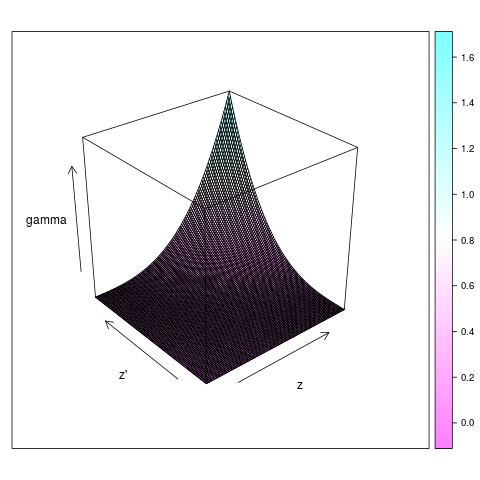
\includegraphics[width=.5\textwidth]{../FIGURES/FigCLADAG-W-graphon} \\
    \end{tabular}
  \end{tabular}
  
 }

%====================================================================
\frame{\frametitle{Some typical graphon functions}

  The graphon function provides a global picture of the network's topology.

  \bigskip \bigskip 
  \centerline{
  \begin{tabular}{ccc}
  'Scale free' & Community & Small world \\
  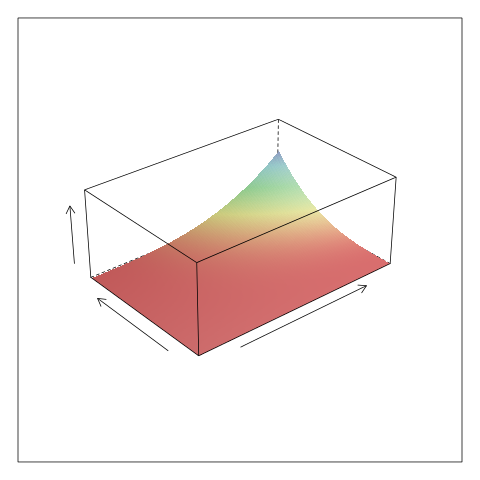
\includegraphics[width=.3\textwidth]{../FIGURES/EDD-ScaleFreeTrueGraphon} &
  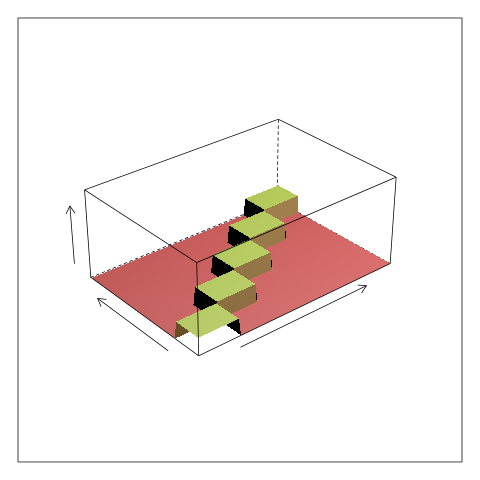
\includegraphics[width=.3\textwidth]{../FIGURES/CommunityTrueGraphon} &
  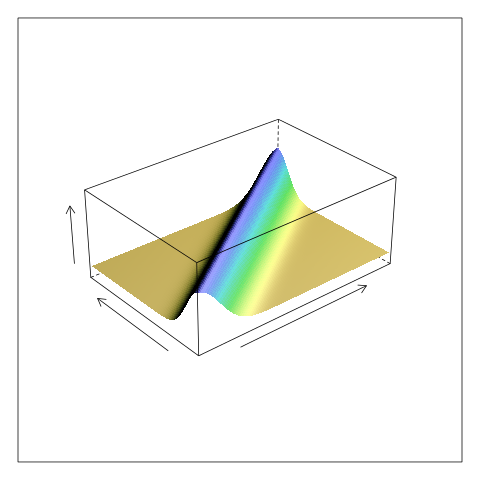
\includegraphics[width=.3\textwidth]{../FIGURES/SmallWorldTrueGraphon} 
  \end{tabular}
  } 
  
  \bigskip \pause
  \paragraph{Remark:} $\gamma(\cdot, \cdot) = $cst \ra ER model

}

%====================================================================
\frame{ \frametitle{Variational Bayes inference of the graphon (1/3)}

  \paragraph{Stochastic Block-model (SBM) as a $W$-graph model.} 

  \bigskip
  \begin{tabular}{cc}
    \hspace{-.02\textwidth}
    \begin{tabular}{p{.5\textwidth}}
	 Latent variables:
	 $$
	 (Z_i) \text{ iid } \sim \Mcal(1, \pi)
	 $$
	 Blockwise constant graphon:
	 $$
	 \gamma(z, z') = \gamma_{k\ell}
	 $$
	 Edges:
	 \begin{eqnarray*}
	 P(Y_{ij} = 1|Z_i, Z_j) & = & \gamma(Z_i, Z_j) \\
	 \logit (~"~) & = & Z_i^\intercal \alpha Z_j \\
	 \alpha & = & \logit(\gamma)
	 \end{eqnarray*}    
	 \end{tabular}
    & 
    \hspace{-.1\textwidth} \pause
    \begin{tabular}{p{.5\textwidth}}
	 Graphon function $\gamma^{SBM}_K(z, z')$ \\
      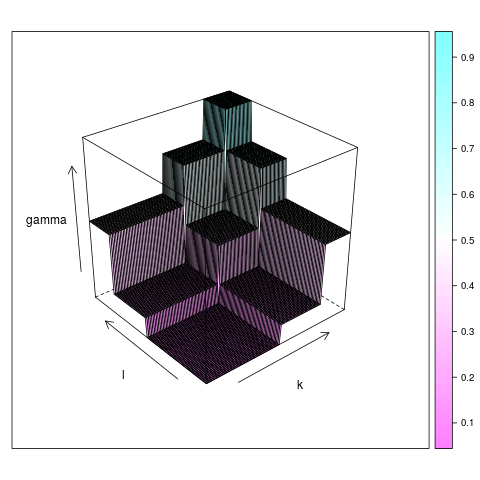
\includegraphics[width=.45\textwidth]{../FIGURES/FigCLADAG-SBM-graphon} \\
    \end{tabular}
  \end{tabular} 

  \ra block widths $= \pi_k$, block heights $\gamma_{k\ell}$
 }

%====================================================================
\frame{ \frametitle{Variational Bayes inference of the graphon (2/3)}

  \begin{tabular}{cc}
    \hspace{-.02\textwidth}
    \begin{tabular}{p{.45\textwidth}}
    \paragraph{VBEM inference of SBM} aims at minimizing
    $$
    KL[\pt(\theta, Z)||p(\theta, Z|Y)]
    $$
    taking $\pt(\theta, Z) = \pt(\theta) \pt(Z)$ \refer{BeG03}. 
    
    \bigskip \bigskip \pause
    Approximate posteriors \refer{LBA11b}:
    \begin{eqnarray*}
    \pt(\pi) & = & \Dcal(\widetilde{\pi}) \\
    \pt(\gamma_{k\ell}) & = & \Beta(\widetilde{\gamma}^0_{k\ell}, \widetilde{\gamma}^1_{k\ell}) \\
    \pt(Z_i) & = & \Mcal(1; \widetilde{\tau}_i) \\
    \end{eqnarray*}
 
%     \bigskip \pause
%     \paragraph{Estimate of $\gamma(u, v)$.} 
%     Due \\
%     to the uncertainty of the $\pi_k$, \\
%     the posterior mean of $\gamma^{SBM}_K$  \\
%     is smooth
%     
%     \bigskip 
%     (Explicit integration using \refer{GoS10})
    \end{tabular}
    & 
    \hspace{-.05\textwidth} \pause
    \begin{tabular}{p{.5\textwidth}}
	 Posterior mean $\Espt[\gamma^{SBM}_K(z, z')]$ \\
      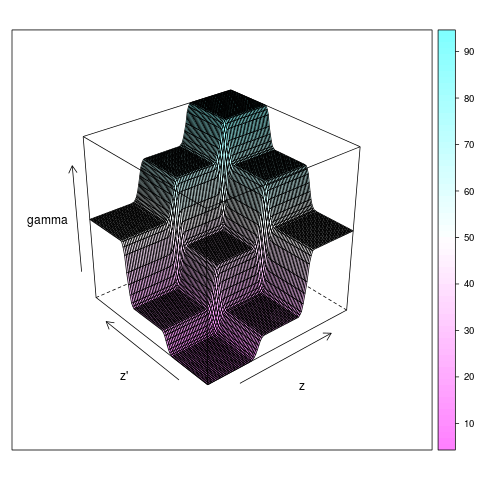
\includegraphics[width=.45\textwidth]{../FIGURES/FigGraphon-SBM-average} \\
    \end{tabular}
  \end{tabular}
  
}

%====================================================================
\frame{ \frametitle{Variational Bayes inference of the graphon (3/3)}

%   The graphon model does not rely on any true $K$.

  \bigskip
  \paragraph{Bayesian model averaging (BMA):} Fit SBM with $K = 1, K_{\max}$ and compute
  $$
  \Esp[\gamma(z, z') | Y] = \sum_K \emphase{p(K|Y)} ~ \Esp[\gamma_K^{SBM}(z, z') | Y]
  $$

%   \bigskip \pause
%   \paragraph{Pushing the variational approximation further:} Consider the model $K$ as an additional hidden variable:
%   $$
%   p(Z, \theta, K|Y) \approx \pt(Z, \theta, K) 
%   := \pt(Z|K) \times \pt(\theta|K) \times \pt(K)  
%   $$
%   
  \bigskip \bigskip \pause
  \paragraph{Variational Bayes model averaging (VBMA) \refer{VMR12}.}
  $$
  p(K|Y) \approx \pt(K) \propto p(K) ~ e^{\log p(Y|K) - KL(K)} = p(K|Y)~ e^{-\emphase{KL(K)}}
  $$ 
  where $KL(K) = KL[\pt(Z, \theta|K) \Vert p(Z,  \theta|Y, K)]$. 
  
  \bigskip \bigskip \bigskip \pause
  \paragraph{VBMA estimate of the graphon \refer{LaR15}:}
  $$
  \Espt[\gamma(z, z')] = \sum_K \emphase{\pt(K)} ~ \Espt[\gamma_K^{SBM}(z, z')].
  $$

}

%====================================================================
\frame{\frametitle{Example: Blog network}

  $n = 196$ blogs. Inferred graphon function:
  $$
  \includegraphics[height=.5\textheight]{../FIGURES/blogd0} 
  $$
  }

%====================================================================
\frame{\frametitle{Example: Tree network}

  $n = 51$ tree species. Inferred graphon function:
  $$
  \includegraphics[height=.5\textheight]{../FIGURES/treed0} 
  $$
  
  \pause
  \begin{itemize}
   \item Graphical representation of the network.
   \item Interpretability...
  \end{itemize}
  }

%====================================================================
%====================================================================
\section{Goodness-of-fit}
\frame{\frametitle{Outline} \tableofcontents[currentsection]}
%====================================================================
\frame{\frametitle{Combined model}

  \bigskip
  \paragraph{Logistic regression:}
  $$
  \logit~P(Y_{ij} = 1) = 
  \beta_0 + \sum_k \beta_k x_{ij}^k
  $$

  \bigskip \bigskip \pause
  \paragraph{Logistic regression + graphon residual term:} $(U_i)$ iid $\sim \Ucal[0, 1]$,
  $$
  \logit~P(Y_{ij} = 1 |U_i, U_j) = 
  \phi(U_i, U_j) + \sum_k \beta_k x_{ij}^k
  $$

  \bigskip \bigskip \pause
  \paragraph{Goodness of fit:} Check if
  $$
  \phi(U_i, U_j) = \cst \qquad (= \beta_0)
  $$
  }

%====================================================================
\frame{\frametitle{Goodness-of-fit as model comparison}

  \paragraph{Logistic model + SBM residual term:} $Z_i \sim \Mcal_K(1; \pi)$, $\alpha: K \times K$,
  $$
  \logit~P(Y_{ij} = 1 | Z_i, Z_j) = Z_i^\intercal \alpha Z_j + \sum_k \beta_k x_{ij}^k.
  $$
  \emphase{Model $M_K =$} logistic regression + $K$-class SBM residual. \\
  (\ra Inference of $\phi$ via averaging over the $M_K$'s).
  
  \bigskip \bigskip \pause
  \paragraph{Goodness of fit:} 
  $$
  \begin{array}{rclcl}
   H_0 & = & \{\text{logistic regression is sufficient}\} & = & M_1 \\
   H_1 & = & \{\text{logistic regression is not sufficient}\} & = & \bigcup_{K > 1} M_K 
  \end{array}
  $$
  GOF is a assessed if
  $$
  p(H_0|Y) = p(M_1|Y) \text{ is large.}
  $$

  }

%====================================================================
\frame{\frametitle{Variational Bayes inference}

  \paragraph{VBEM:} A global variational Bayes EM algorithm can be designed to obtain all needed (approximate) posteriors:
  $$
  \pt(\beta|K), \qquad \pt(\pi|K), \qquad \pt(\alpha|K), \qquad \pt(Z|K), \qquad \pt(K).
  $$
  
  \bigskip \pause
  \paragraph{Posterior quantities of interest:}
  \begin{itemize}
   \item Goodness of fit criterion:
   $$
   p(H_0|Y) \approx \Pt(K=1)
   $$
   \item Residual graphon:
   $$
   \widehat{\phi}(U_i, U_j) = \sum_K \pt(K) ~ \Espt[\phi^{SBM}_K(U_i, U_j)]
   $$
  \end{itemize}

  
  }

%====================================================================
%====================================================================
\section{Illustrations}
\frame{\frametitle{Outline} \tableofcontents[currentsection]}
%====================================================================
\frame{\frametitle{Blog network}

  $n = 196$ species, 3 covariates, density $= .07$ 

  \bigskip
  \begin{tabular}{cc}
    \begin{tabular}{p{.5\textwidth}}
	 Inferred graphon (no covariate) \\ ~\\
	 \includegraphics[height=.4\textheight]{../FIGURES/blogd0} \\ ~\\
	 ~
    \end{tabular}
    & 
    \hspace{-.05\textwidth}
    \begin{tabular}{p{.5\textwidth}}
	 Residual graphon (3 covariates) \\ ~\\
	 \includegraphics[height=.4\textheight]{../FIGURES/blogd3} \\ ~\\
	 $\Pt(H_0) \simeq 10^{-172}$
    \end{tabular}
  \end{tabular}
  }

%====================================================================
\frame{\frametitle{Tree network}

  $n = 51$ species, 3 covariates, density $= .54$ 

  \bigskip
  \begin{tabular}{cc}
    \begin{tabular}{p{.5\textwidth}}
	 Inferred graphon (no covariate) \\ ~\\
	 \includegraphics[height=.4\textheight]{../FIGURES/treed0} \\ ~\\
	 ~
    \end{tabular}
    & 
    \hspace{-.05\textwidth}
    \begin{tabular}{p{.5\textwidth}}
	 Residual graphon (3 covariates) \\ ~\\
	 \includegraphics[height=.4\textheight]{../FIGURES/treed3} \\ ~\\
	 $\Pt(H_0) \simeq 10^{-152}$
    \end{tabular}
  \end{tabular}
  }

%====================================================================
\frame{\frametitle{Florentine business}

  $n = 16$ family, 3 covariates, density $= .12$ 

  \bigskip
  \begin{tabular}{cc}
    \begin{tabular}{p{.5\textwidth}}
	 Inferred graphon (no covariate) \\ ~\\
	 \includegraphics[height=.4\textheight]{../FIGURES/businessd0} \\ ~\\
	 ~
    \end{tabular}
    & 
    \hspace{-.05\textwidth}
    \begin{tabular}{p{.5\textwidth}}
	 Residual graphon (3 covariates) \\ ~\\
	 \includegraphics[height=.4\textheight]{../FIGURES/businessd3} \\ ~\\
	 $\Pt(H_0) = .99$
    \end{tabular}
  \end{tabular}
  }

%====================================================================
%====================================================================
\section{Discussion}
\frame{\frametitle{Outline} \tableofcontents[currentsection]}
%====================================================================
\frame{\frametitle{Discussion}

  \paragraph{Summary:}
  \begin{itemize}
   \item A generic logistic regression model with a network oriented residual term.
   \item The detour through SBM provides a natural goodness-of-fit criterion.
  \end{itemize}

  \bigskip \bigskip \pause
  \paragraph{Future work:}
  \begin{itemize}
   \item All this strongly relies on variational Bayes approximation of the posteriors. \item VB \& VBEM are quite accurate for logistic regression and SBM separately.
   \item No clue about their accuracy in the combined model.
   \item Use importance sampling?
   \end{itemize}


}

%====================================================================
\frame[allowframebreaks]{ \frametitle{References}
{\tiny
  \bibliography{/home/robin/Biblio/ARC,/home/robin/Biblio/BibGene}
  %\bibliographystyle{/home/robin/LATEX/Biblio/astats}
  \bibliographystyle{plain}
  }
}

%====================================================================
%====================================================================
\end{document}
%====================================================================
%====================================================================

  \begin{tabular}{cc}
    \begin{tabular}{p{.5\textwidth}}
    \end{tabular}
    & 
    \hspace{-.02\textwidth}
    \begin{tabular}{p{.5\textwidth}}
    \end{tabular}
  \end{tabular}

